\documentclass[8pt,dvipsnames]{beamer}
\usepackage[T1]{fontenc}
\usepackage{libertinus}
\usepackage{amsmath}
\usepackage[most]{tcolorbox}
\usepackage{graphicx}

\usepackage{hyperref}
%python 
\usepackage{listings}
% Default fixed font does not support bold face
\DeclareFixedFont{\ttb}{T1}{txtt}{bx}{n}{8} % for bold
\DeclareFixedFont{\ttm}{T1}{txtt}{m}{n}{8}  % for normal

% Custom colors
\usepackage{color}
\definecolor{deepblue}{rgb}{0,0,0.5}
\definecolor{deepred}{rgb}{0.6,0,0}
\definecolor{deepgreen}{rgb}{0,0.5,0}

\usepackage{listings}

% Python style for highlighting
\newcommand\pythonstyle{\lstset{
		language=Python,
		basicstyle=\ttm,
		morekeywords={self},              % Add keywords here
		keywordstyle=\ttb\color{deepblue},
		emph={MyClass,__init__},          % Custom highlighting
		emphstyle=\ttb\color{deepred},    % Custom highlighting style
		stringstyle=\color{deepgreen},
		frame=tb,                         % Any extra options here
		showstringspaces=false
}}


% Python environment
\lstnewenvironment{python}[1][]
{
	\pythonstyle
	\lstset{#1}
}
{}

% Python for external files
\newcommand\pythonexternal[2][]{{
		\pythonstyle
		\lstinputlisting[#1]{#2}}}

% Python for inline
\newcommand\pythoninline[1]{{\pythonstyle\lstinline!#1!}}

\usepackage{xcolor}  
\newcommand{\cb}[1]{{\color{CadetBlue}#1}}

\usepackage{pgfplots}
\pgfplotsset{compat=newest}
\setlength{\parskip}{0.5em}

\usepackage{setspace}
\setstretch{1.25}  
\usetheme{Singapore}
\setbeamertemplate{navigation symbols}{}


\title{CSE574 Introduction to Machine Learning}
\subtitle{Neural Networks 1}
\author{Jue Guo}
\institute{University at Buffalo}
\date{\today}

\begin{document}
\begin{frame}
	\titlepage
\end{frame}
\begin{frame}
	\frametitle{Outline}
	\tableofcontents
\end{frame}

\section{Neural Networks}
\begin{frame}{Neural Networks}
	First of all, you already know what a neural network is, and you already know how to build such a model.
	\begin{itemize}
		\item Yes, it's logistic regression! As a matter of fact, the logistic regression model, or rather its generalization for multiclass classification, called the softmax regression model, is a standard unit in a neural network.
	\end{itemize}
	A neural network (NN), just like a regression or an SVM model, is a mathematical function:

	$$
		y=f_{N N}(\mathbf{x}) \text {. }
	$$

	The function $f_{N N}$ has a particular form: it's a nested function.
\end{frame}

\begin{frame}
	You have probably already heard of neural network layers. So, for a 3-layer neural network that returns a scalar, $f_{N N}$ looks like this:

	$$
		y=f_{N N}(\mathbf{x})=f_{3}\left(\boldsymbol{f}_{2}\left(\boldsymbol{f}_{1}(\mathbf{x})\right)\right)
	$$

	In the above equation, $f_{1}$ and $f_{2}$ are vector functions of the following form:

	$$
		\boldsymbol{f}_{l}(\mathbf{z}) \stackrel{\text { def }}{=} \boldsymbol{g}_{l}\left(\mathbf{W}_{l} \mathbf{z}+\mathbf{b}_{l}\right)
	$$
	where $l$ is called the layer index and can span from 1 to any number of layers. The function $\boldsymbol{g}_{l}$ is called an \textbf{activation function}. It is a fixed, usually nonlinear function chosen by the data analyst before the learning is started. The parameters $\mathbf{W}_{l}$ (a matrix) and $\mathbf{b}_{l}$ (a vector) for each layer are learned using the familiar gradient descent by optimizing, depending on the task, a particular cost function (such as MSE).

	Compared with the equation for logistic regression, where you replace $\boldsymbol{g}_{l}$ by the sigmoid function, and you will not see any difference. The function $f_{3}$ is a scalar function for the regression task, but can also be a vector function depending on your problem.
\end{frame}

\begin{frame}
	You may probably wonder why a matrix $\mathbf{W}_{l}$ is used and not a vector $\mathbf{w}_{l}$.
	\begin{itemize}
		\item The reason is that $\boldsymbol{g}_{l}$ is a vector function. Each row $\mathbf{w}_{l, u}$ ( $u$ for unit) of the matrix $\mathbf{W}_{l}$ is a vector of the same dimensionality as $\mathbf{z}$. Let $a_{l, u}=\mathbf{w}_{l, u} \mathbf{z}+b_{l, u}$.
	\end{itemize}
	The output of $\boldsymbol{f}_{l}(\mathbf{z})$ is a vector $\left[g_{l}\left(a_{l, 1}\right), g_{l}\left(a_{l, 2}\right), \ldots, g_{l}\left(a_{l, s i z e_{l}}\right)\right]$, where $g_{l}$ is some scalar function \footnote[frame]{A scalar function outputs a scalar, that is a simple number and not a vector.}, and size $_{l}$ is the number of units in layer $l$. To make it more concrete, let's consider one architecture of neural networks called \textbf{multilayer perceptron} and often referred to as a \textbf{vanilla neural network}.
\end{frame}

\subsection{Multilayer Perceptron Example}
\begin{frame}{Multilayer Perceptron Example}
	We have a closer look at one particular configuration of neural networks called \textbf{feed-forward neural networks} (FFNN), and more specifically the architecture called a \textbf{multilayer perceptron} (MLP).
	\begin{itemize}
		\item 	As an illustration, let's consider an MLP with three layers. Our network takes a two-dimensional feature vector as input and outputs a number. This FFNN can be a regression or a classification model, depending on the activation function used in the third, output layer.
	\end{itemize}
\end{frame}

\begin{frame}
	The neural network is represented graphically as a connected combination of \textbf{units} logically organized into one or more \textbf{layers}.
	\begin{itemize}
		\item Each unit is represented by either a circle or a rectangle. The inbound arrow represents an input of a unit and indicates where this input came from. The outbound arrow indicates the output of a unit.
	\end{itemize}
	\begin{figure}
		\centering
		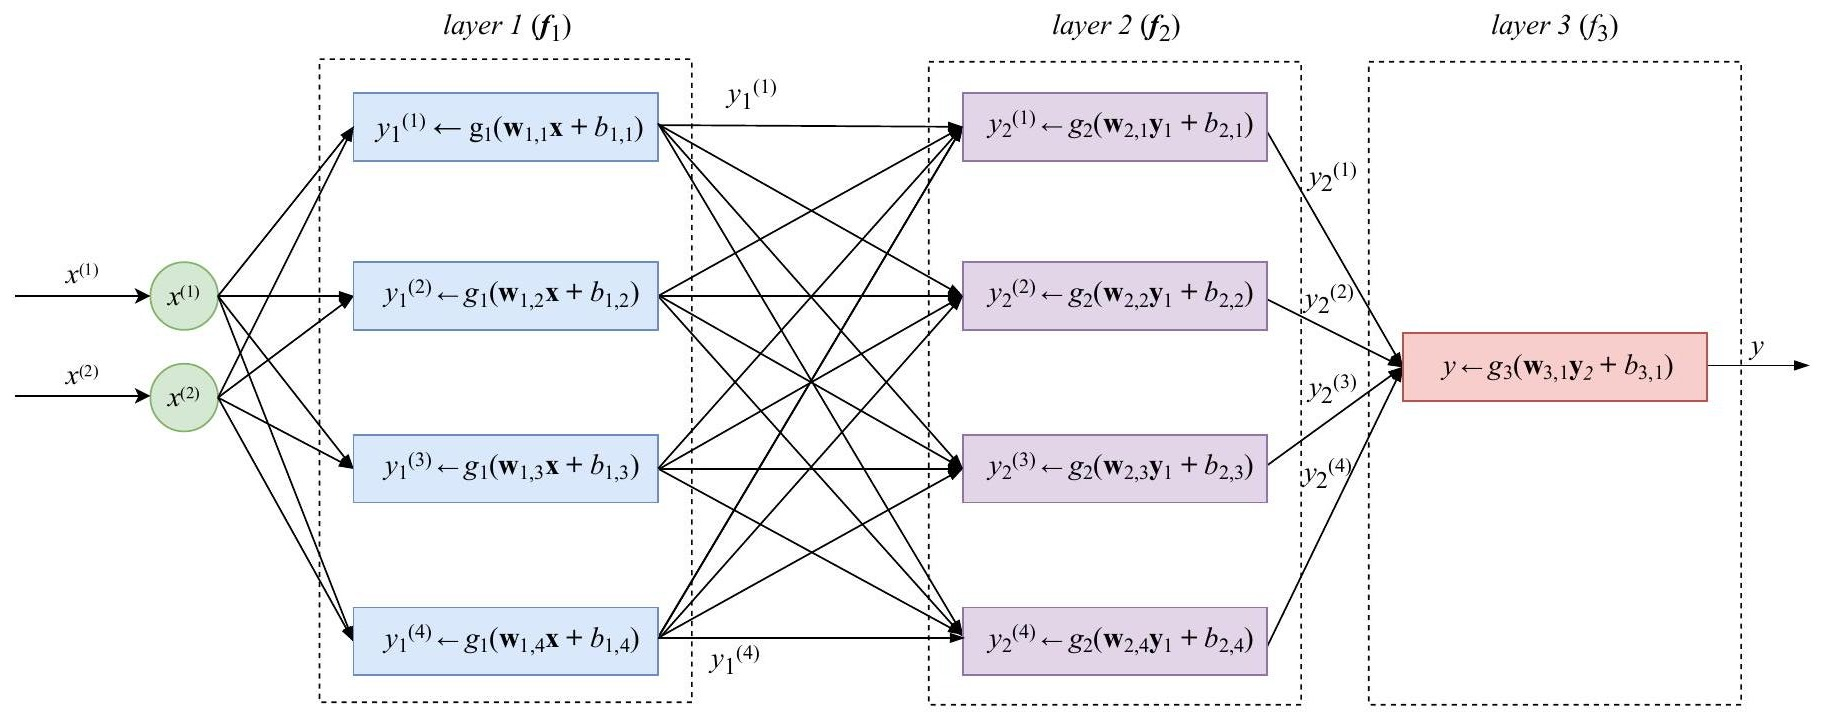
\includegraphics[width=\textwidth]{imgs/nn_1.jpeg}
		\caption{A multi-layer perceptron with two-dimensional input, two layers with four units and one output layer with one unit.}
	\end{figure}
\end{frame}

\begin{frame}
	The output of each unit is the result of the mathematical operation written inside the rectangle. Circle units don't do anything with the input; they just send their input directly to the output.

	The following happens in each rectangle unit.
	\begin{enumerate}
		\item Firstly, all inputs of the unit are joined together to form an input vector.
		\item Then the unit applies a linear transformation to the input vector, exactly like linear regression model does with its input feature vector.
		\item Finally, the unit applies an activation function $g$ to the result of the linear transformation and obtains the output value, a real number.
	\end{enumerate}
	In a vanilla FFNN, the output value of a unit of some layer becomes an input value of each of the units of the subsequent layer.
\end{frame}

\begin{frame}
	\begin{figure}
		\centering
		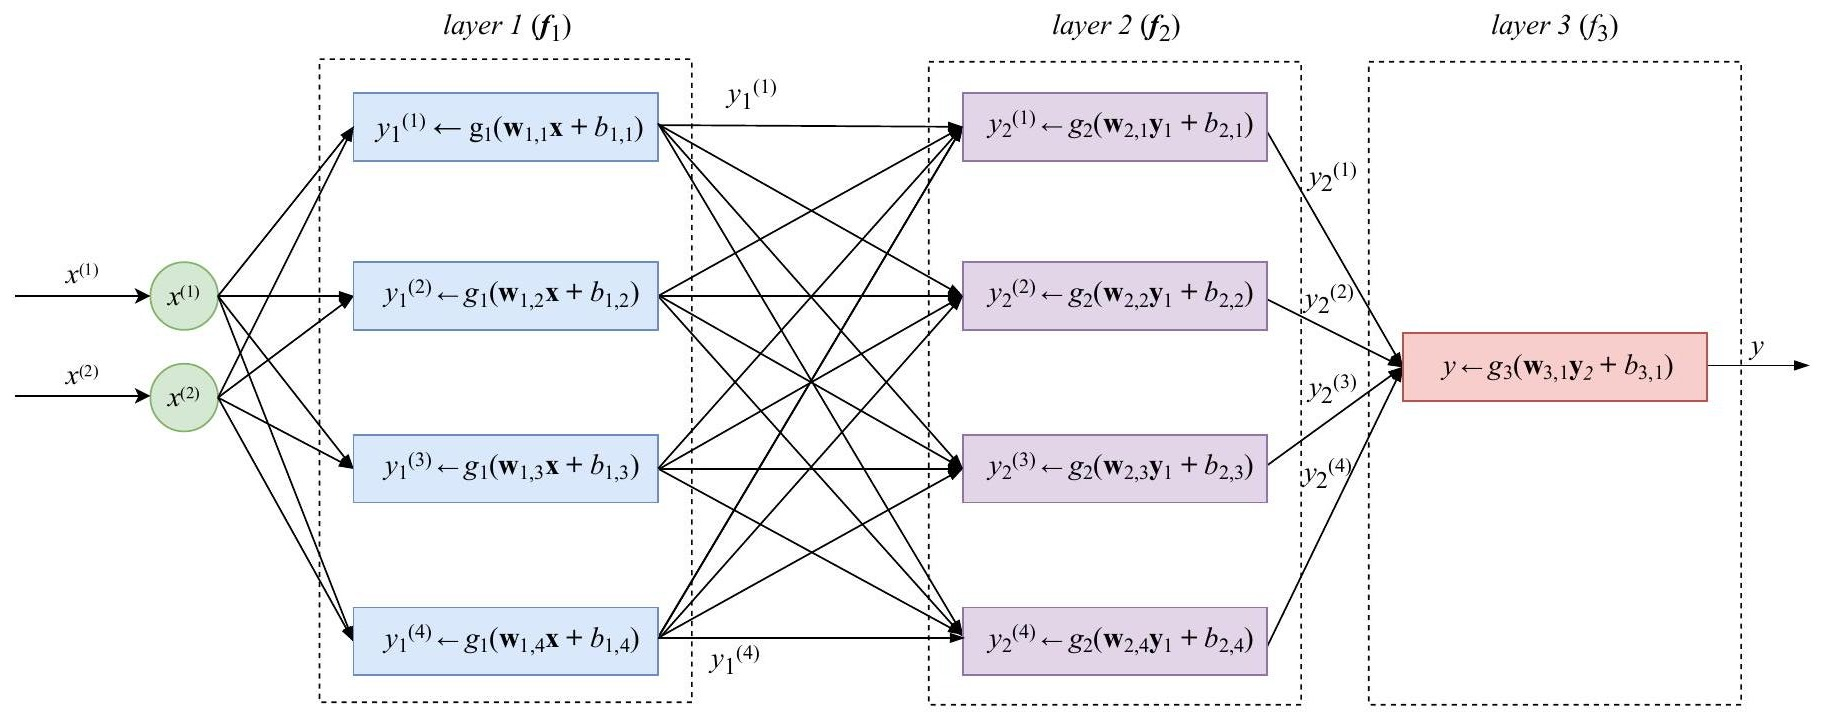
\includegraphics[width=0.6\textwidth]{imgs/nn_1.jpeg}
		\caption{A multi-layer perceptron with two-dimensional input, two layers with four units and one output layer with one unit.}
	\end{figure}
	The activation function $g_{l}$ has one index: $l$, the index of the layer the unit belongs to. Usually, all units of a layer use the same activation function, but it's not a rule.
	\begin{itemize}
		\item Each layer can have a different number of units.
		\item Each unit has its parameters $\mathbf{w}_{l, u}$ and $b_{l, u}$, where $u$ is the index of the unit, and $l$ is the index of the layer.
	\end{itemize}
	The vector $\mathbf{y}_{l-1}$ in each unit is defined as $\left[y_{l-1}^{(1)}, y_{l-1}^{(2)}, y_{l-1}^{(3)}, y_{l-1}^{(4)}\right]$. The vector $\mathbf{x}$ in the first layer is defined as $\left[x^{(1)}, \ldots, x^{(D)}\right]$.
\end{frame}

\begin{frame}
	\begin{figure}
		\centering
		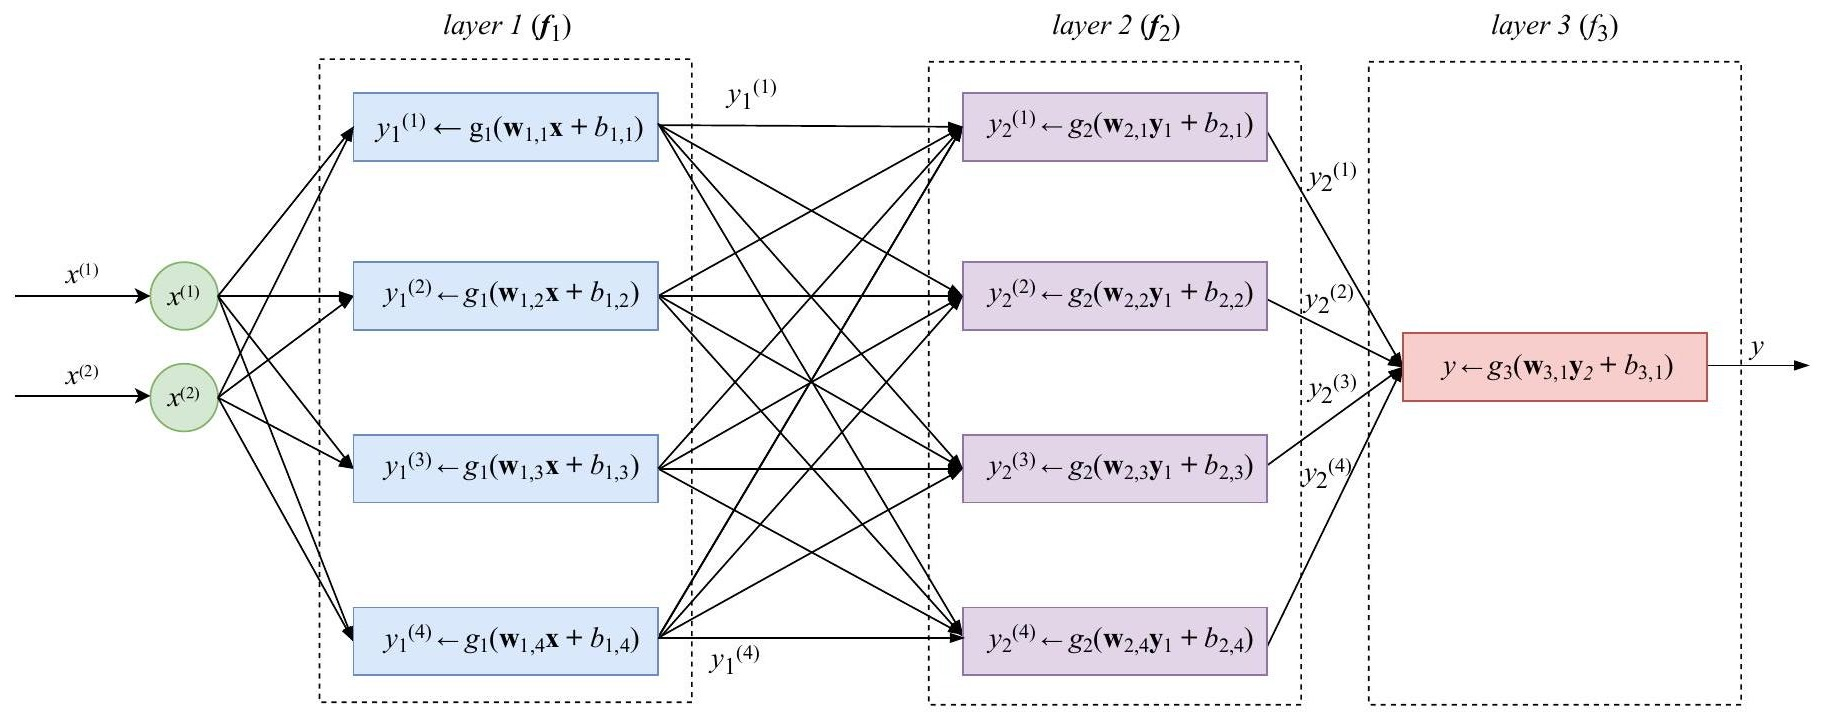
\includegraphics[width=\textwidth]{imgs/nn_1.jpeg}
		\caption{A multi-layer perceptron with two-dimensional input, two layers with four units and one output layer with one unit.}
	\end{figure}
	In multilayer perceptron all outputs of one layer are connected to each input of the succeeding layer. This architecture is called \textbf{fully-connected}. A neural network can contain \textbf{fully-connected layers}. Those are the layers whose units receive as inputs the outputs of each of the units of the previous layer.
\end{frame}

\subsection{Feed-Forward Neural Network Architecture}
\begin{frame}{Feed-Forward Neural Network Architecture}
	If we want to solve a regression or a classification problem, the last (the rightmost) layer of a neural network usually contains only one unit.
	\begin{itemize}
		\item If the activation function $g_{\text {last }}$ of the last unit is linear, then the neural network is a regression model.
		\item If the $g_{\text {last }}$ is a logistic function, the neural network is a binary classification model.
	\end{itemize}
	The data analyst can choose any mathematical function as $g_{l, u}$, assuming it's differentiable \footnote[frame]{The function has to be differentiable across its whole domain or in the majority of the points of its domain. For example, ReLU is not differentiable at 0 .}. The latter property is essential for gradient descent used to find the values of the parameters $\mathbf{w}_{l, u}$ and $b_{l, u}$ for all $l$ and $u$.
	\begin{itemize}
		\item The primary purpose of having nonlinear components in the function $f_{N N}$ is to allow the neural network to approximate nonlinear functions.
	\end{itemize}
	Without nonlinearities, $f_{N N}$ would be linear, no matter how many layers it has. The reason is that $\mathbf{W}_{l} \mathbf{z}+\mathbf{b}_{l}$ is a linear function and a linear function of a linear function is also linear.
\end{frame}

\begin{frame}{Activation Functions}
	Popular choices of activation functions are the logistic function, already known to you, as well as TanH and ReLU.
	\begin{itemize}
		\item The former is the hyperbolic tangent function, similar to the logistic function but ranging from -1 to 1 (without reaching them).
		\item The latter is the rectified linear unit function, which equals to zero when its input $z$ is negative and to $z$ otherwise:
	\end{itemize}
	$$
		\begin{gathered}
			\tanh (z)=\frac{e^{z}-e^{-z}}{e^{z}+e^{-z}}, \\
			\operatorname{relu}(z)= \begin{cases}0 & \text { if } z<0    \\
             z & \text { otherwise }\end{cases}
		\end{gathered}
	$$
\end{frame}

\begin{frame}

	\begin{columns}
		\column{0.5\textwidth}
		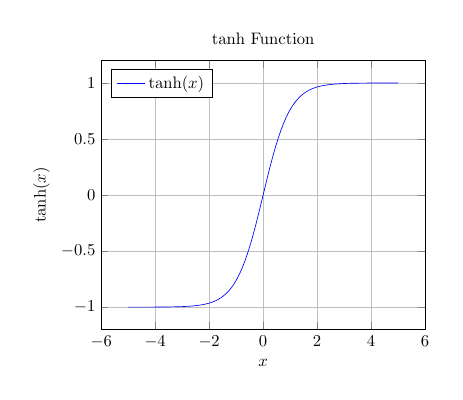
\begin{tikzpicture}[scale=0.6]
			\begin{axis}[
					title={tanh Function},
					xlabel={$x$},
					ylabel={$\text{tanh}(x)$},
					grid=major,
					legend entries={$\text{tanh}(x)$},
					legend pos=north west,
				]
				\addplot[domain=-5:5, samples=100, color=blue]{tanh(x)};
			\end{axis}
		\end{tikzpicture}
		\column{0.5\textwidth}
		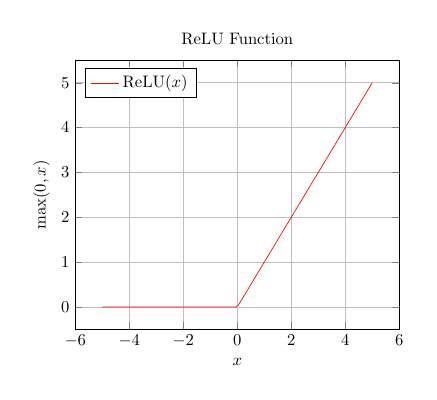
\begin{tikzpicture}[scale=0.6]
			\begin{axis}[
					title={ReLU Function},
					xlabel={$x$},
					ylabel={$\max(0, x)$},
					grid=major,
					legend entries={$\text{ReLU}(x)$},
					legend pos=north west,
				]
				\addplot[domain=-5:5, samples=100, color=red]{max(0, x)};
			\end{axis}
		\end{tikzpicture}
	\end{columns}
\end{frame}

\end{document}